\section{Phân tích yêu cầu hệ thống}
Hệ thống quản lý cán bộ tầm trung với số lượng khoảng 1200 cán bộ. Nhiệm vụ của hệ thống thông tin phòng Tổ chức - Hành chính được tóm gọn trong các chức năng sau: 
\subsection{Quản lý cán bộ}
Quản lý cán bộ là chức năng quan trọng nhất và cần phải có của phòng Tổ chức - Hành chính, cũng như là hệ thống thông tin phòng Tổ chức - Hành chính. Chức năng quản lý cán bộ sẽ bao gồm:
\begin{itemize}
    \item Hiển thị danh sách toàn bộ cán bộ, công chức viên chức của nhà trường.
    \item Quản lý thông tin của cán bộ: thông tin bao gồm các thông tin cá nhân và một số thông tin của người thân. Hệ thống cho phép chỉnh sửa và cập nhật khi thông tin có thay đổi.
    \item Khi có nhân viên mới bắt đầu làm việc tại trường, cán bộ đó sẽ được thêm vào hệ thống để dễ quản lý thông tin.
    \item Thông tin của cán bộ được xuất ra dưới định dạng sơ yếu lý lịch theo mẫu 2C-BNV/2008 để thuận tiện cho công việc.
\end{itemize}
\subsection{Quản lý các loại hồ sơ, bằng cấp của cán bộ}
Mỗi cán bộ sẽ có những hồ sơ cá nhân như:
\begin{itemize}
    \item Bằng cấp, chứng chỉ: Bằng tiến sĩ, thạc sĩ, bằng đại học.
    \item Hồ sơ cá nhân: Hồ sơ xin việc, lý lịch viên chức.
    \item Hồ sơ bảo hiểm xã hội.
    \item Quyết định bổ nhiệm; quyết định đào tạo, bồi dưỡng,...
\end{itemize}

Hệ thống hỗ trợ lưu trữ các loại hồ sơ của cán bộ dưới dạng tệp tin. Bên cạnh đó, hệ thống còn cho phép thêm mới, xóa bỏ bất kỳ hồ sơ nào.
\subsection{Quản lý quá trình nghiệp vụ}
Bên cạnh quản lý cán bộ hệ thống phải còn đảm nhiệm chức năng quan trọng là quản lý quá trình nghiệp vụ của cán bộ. Những quá trình nghiệp vụ hiện có ở trường Đại học Bách Khoa: 
\begin{itemize}
    \item Quá trình đào tạo: Bao gồm các thông tin liên quan đến quá trình đào tạo của một cán bộ như:
        \subitem - Danh tính cán bộ được đào tạo
        \subitem - Số hiệu quyết định, ngày quyết định đào tạo
        \subitem - Thời gian đào tạo
        \subitem - Cấp đào tạo, chuyên ngành đào tạo, cơ sở đào tạo
    \item Quá trình chuyển ngạch: Bao gồm các thông tin liên quan đến quá trình chuyển ngạch của một cán bộ như:
        \subitem - Danh tính cán bộ chuyển ngạch
        \subitem - Số hiệu quyết định, ngày quyết định chuyển ngạch
        \subitem - Thông tin ngạch cũ và ngạch mới
        \subitem - Bậc lương, hệ số lương
    \item Quá trình phụ cấp độc hại: Bao gồm các thông tin về quá trình hưởng phụ cấp do làm việc trong môi trường độc hại:
        \subitem - Danh tính cán bộ được hưởng phụ cấp
        \subitem - Số hiệu quyết định, ngành quyết định được hưởng phụ cấp
        \subitem - Thời gian được hưởng phụ cấp
        \subitem - Môi trường độc hại và mức phụ cấp được hưởng
    \item Quá trình công tác nước ngoài: Bao gồm các thông tin về những lần đi công tác nước ngoài của cán bộ:
        \subitem - Danh tính cán bộ đi công tác
        \subitem - Số hiệu quyết định, ngày quyết định cho cán bộ đi công tác nước ngoài
        \subitem - Thời gian đi công tác: từ ngày, đến ngày, ngày phải về và ngày về thực tế
        \subitem - Mục đích đi công tác nước ngoài, nước đến và nơi đến
        \subitem - Kinh phí đi, lương được hưởng trong thời gian đi công tác
    \item Quá trình công tác trong nước: Bao gồm các thông tin về những lần đi công tác trong nước của cán bộ:
        \subitem - Danh tính cán bộ đi công tác
        \subitem - Số hiệu quyết định, ngày quyết định
        \subitem - Nơi công tác, mục đích
        \subitem - Thời gian đi công tác, phương tiện đi lại
        \subitem - Nội dung công tác
    \item Quá trình chức danh khoa học: Bao gồm thông tin các quá trình được bổ nhiệm chức danh khoa học của cán bộ:
        \subitem - Danh tính cán bộ được bổ nhiệm
        \subitem - Số hiệu quyết định, ngày quyết định bổ nhiệm chức danh
        \subitem - Chức danh khoa học được bổ nhiệm: Giáo sư, phó giáo sư, viện sĩ
    \item Quá trình chức vụ: Bao gồm thông tin các quá trình bổ nhiệm chức vụ mới của cán bộ:
        \subitem - Danh tính cán bộ được bổ nhiệm
        \subitem - Số hiệu quyết định, ngày quyết định bổ nhiệm, ngày bổ nhiệm chức vụ
        \subitem - Chức vụ được bổ nhiệm
        \subitem - Bộ môn chính, đơn vị chính
    \item Quá trình khen thưởng: Bao gồm thông tin các quá trình được khen thưởng của cán bộ
        \subitem - Danh tính cán bộ được bổ nhiệm
        \subitem - Số hiệu quyết định, ngày quyết định khen thưởng
        \subitem - Danh hiệu khen thưởng, cấp khen thưởng
        \subitem - Năm khen thưởng
    \item Quá trình phụ cấp thâm niên nhà giáo: Bao gồm các thông tin hưởng phụ cấp thâm niên nhà giáo của cán bộ
        \subitem - Danh tính cán bộ được hưởng phụ cấp thâm niên
        \subitem - Thời gian được hưởng phụ cấp
        \subitem - Mức phụ cấp được hưởng
    \item Quá trình chức danh nghề nghiệp: Bao gồm các thông tin bổ nhiệm chức danh nghề nghiệp của cán bộ
        \subitem - Danh tính cán bộ được bổ nhiệm chức danh nghề nghiệp mới
        \subitem - Số hiệu quyết đinh, ngày quyết định, ngày bổ nhiệm chức danh nghề nghiệp
        \subitem - Chức danh nghề nghiệp được bổ nhiệm
    \item Quá trình nghỉ: Bao gồm những thông tin về nghỉ phép của cán bộ
        \subitem - Danh tính cán bộ
        \subitem - Số hiệu quyết định, ngày quyết định nghỉ
        \subitem - Số hiệu quyết định tiếp nhận, ngày quyết định tiếp nhận, ngày tiếp nhận
        \subitem - Thời gian nghỉ
        \subitem - Lí do nghỉ: Nghỉ ốm, nghỉ thai sản
    \item Quá trình tập sự: Bao gồm thông tin tập sự của cán bộ
        \subitem - Danh tính cán bộ tập sự
        \subitem - Quyết định, ngày quyết định tập sự
        \subitem - Thời gian tập sự
        \subitem - Tỷ lệ lương tập sự
    \item Quá trình ký hợp đồng: Bao gồm thông tin về những lần ký hợp đồng của cán bộ
        \subitem - Danh tính cán bộ ký hợp đồng
        \subitem - Số hợp đồng
        \subitem - Đối tượng cán bộ, loại hợp đồng
        \subitem - Thời hạn của hợp đồng
        \subitem - Ngày ký hợp đồng
    \item Quá trình lương: Bap gồm các thông tin về quá trình thay đổi lương của cán bộ
        \subitem - Danh tính cán bộ
        \subitem - Số quyết định, ngày quyết định lương
        \subitem - Ngạch lương, bậc lương, hệ số lương
        \subitem - Mốc nâng lương, ngày hưởng lương
    \item Quá trình kỷ luật: Bao gồm các thông tin về kỷ luật của cán bộ
        \subitem - Danh tính cán bộ bị kỷ luật
        \subitem - Số quyết định, ngày quyết định kỷ luật
        \subitem - Hình thức kỷ luật và hình thức kỷ luật đi kèm
        \subitem - Lí do bị kỷ luật
        \subitem - Năm kỷ luật
\end{itemize}

Đối với mỗi quá trình nghiệp vụ trên, hệ thống cho phép thêm thông tin mới, chỉnh sửa thông tin, cũng như là xóa thông tin đã tồn tại
\subsection{Quản lý yêu cầu của cán bộ}
Đối với mỗi quá trình nghiệp vụ, khi cán bộ nhà trường có nhu cầu thêm mới, chỉnh sửa hoặc xóa một quá trình nghiệp vụ của bản thân thì hệ thống sẽ tạo yêu cầu. Yêu cầu này cần phải được duyệt bởi phòng Tổ chức - Hành chính. Sau khi yêu cầu được duyệt, quá trình của cán bộ tạo yêu cầu sẽ được cập nhật.
\subsection{Quản lý danh mục}
Để việc nhập các thông tin quá trình một cách dễ dàng nhất, hệ thống cung cấp các danh mục thông tin liên quan. Một số danh mục như sau:
\begin{itemize}
    \item Danh mục quốc gia
    \item Danh mục phường xã, quận huyện, tỉnh thành phố
    \item Danh mục bộ môn, đơn vị
    \item Danh mục chức danh khoa học, chức danh nghề nghiệp
    \item Danh mục khen thưởng, hình thức kỷ luật, hình thức kỷ luật kèm theo
    \item Danh mục mục đích đi nước ngoài, mục đích công tác trong nước
    \item Danh mục đối tượng cán bộ, loại hợp đồng
\end{itemize}

Đối với mỗi danh mục trên, hệ thống cho phép thêm mới thông tin cho danh mục, chỉnh sửa thông tin của danh mục hoặc xóa thông tin danh mục không còn cần thiết nữa.
\subsection{Xem thống kê các số liệu tổng quát của hệ thống}
Hệ thống cần phải cung cấp cái nhìn tổng quát về những số liệu thuộc về phòng Tổ chức - Hành chính:
\begin{itemize}
    \item Số lượng cán bộ theo từng khoa, từng đơn vị
    \item Tỉ lệ giới tính của cán bộ
    \item Số lượng cán bộ mới trong tháng
    \item Số lượng yêu cầu được tạo trong tháng
    \item Số lượng các yêu cầu chia theo trạng thái
\end{itemize}
\subsection{Gửi thông báo bằng email}
Hệ thống gửi thông báo qua email khi có những hành động liên quan đến các yêu cầu của cán bộ:
\begin{itemize}
    \item Cán bộ tạo một yêu cầu mới
    \item Yêu cầu đã được duyệt, yêu cầu bị từ chối duyệt
    \item Yêu cầu có bình luận mới
\end{itemize}
\section{Tổng quát kiến trúc hệ thống}
\indent 
    Hệ thống được xây dựng theo mô hình MVC kết hợp với REST API (RESTful). Ngoài ra để xử lý các tác vụ real time, nhóm sử dụng lớp Socket.io ở giữa tầng View và Controller.
Vận dụng kiến trúc REST API trong hệ thống:
Các API trong hệ thống Tổ chức-Hành chính được thiết kế theo các nguyên tắc chung, nhất quán giữa các module.
\begin{itemize}
    \item API được đặt tên theo quy định chung, phù hợp với công dụng, quyền của API, thống nhất giữa các module.
    \begin{itemize}
        \item \textit{``/api/tchc/qua-trinh/dao-tao/all''}, \textit{``/api/tchc/qua-trinh/khen-thuong/all''}: API lấy tất cả dữ liệu của một bảng quá trình (đào tạo, khen thưởng). Ta có thể thấy các API có cấu trúc thống nhất với nhau với các bảng khác.
        \item \textit{``/api/tchc/qua-trinh/dao-tao/item/:id''}, \textit{``/api/user/qua-trinh/dao-tao/item/:id''}: API lấy dữ liệu của bảng quá trình đào tạo theo ID. API thứ nhất dùng cho cán bộ phòng Tổ chức - Hành chính, API thứ hai dành cho người dùng của hệ thống.
    \end{itemize}
    \item Sử dụng các phương thức HTTP (GET, POST, PUT, DELETE) để truy cập và xử lý dữ liệu.
    \begin{itemize}
        \item  \textit{POST /api/tchc/qua-trinh/dao-tao/all}: cách dùng API để lấy dữ liệu.
        \item  \textit{POST /api/tchc/qua-trinh/dao-tao}: cách dùng API để thêm dữ liệu.
        \item  \textit{PUT /api/tchc/qua-trinh/dao-tao}: cách dùng API để sửa đổi dữ liệu.
        \item  \textit{DELETE /api/tchc/qua-trinh/dao-tao}: cách dùng API để xoá dữ liệu.
    \end{itemize}
    \item Dữ liệu được server trả về theo định dạng JSON.
    \item Server trả về các HTTP code phù hợp.
    \begin{itemize}
        \item  400 Invalid parameter: Trả về lỗi này khi client gửi yêu cầu sai cú pháp.
        \item  403 Can not access data: Trả về lỗi này khi client không có quyền truy cập dữ liệu.
        \item  404 Not found: Trả về lỗi này khi server không tìm thấy dữ liệu client yêu cầu.
    \end{itemize}
\end{itemize}

Nhận thấy mô hình MVC có nhiều ưu điểm và phù hợp với hệ thống (trình bày ở mục 2.1 Mô hình Model-View-Controller) nên nhóm đã sử dụng mô hình này trong thiết kế kiến trúc hệ thống.\\

Vận dụng mô hình MVC trong hệ thống phòng Tổ chức - Hành chính:
\begin{center}
  \captionsetup{type=figure}
  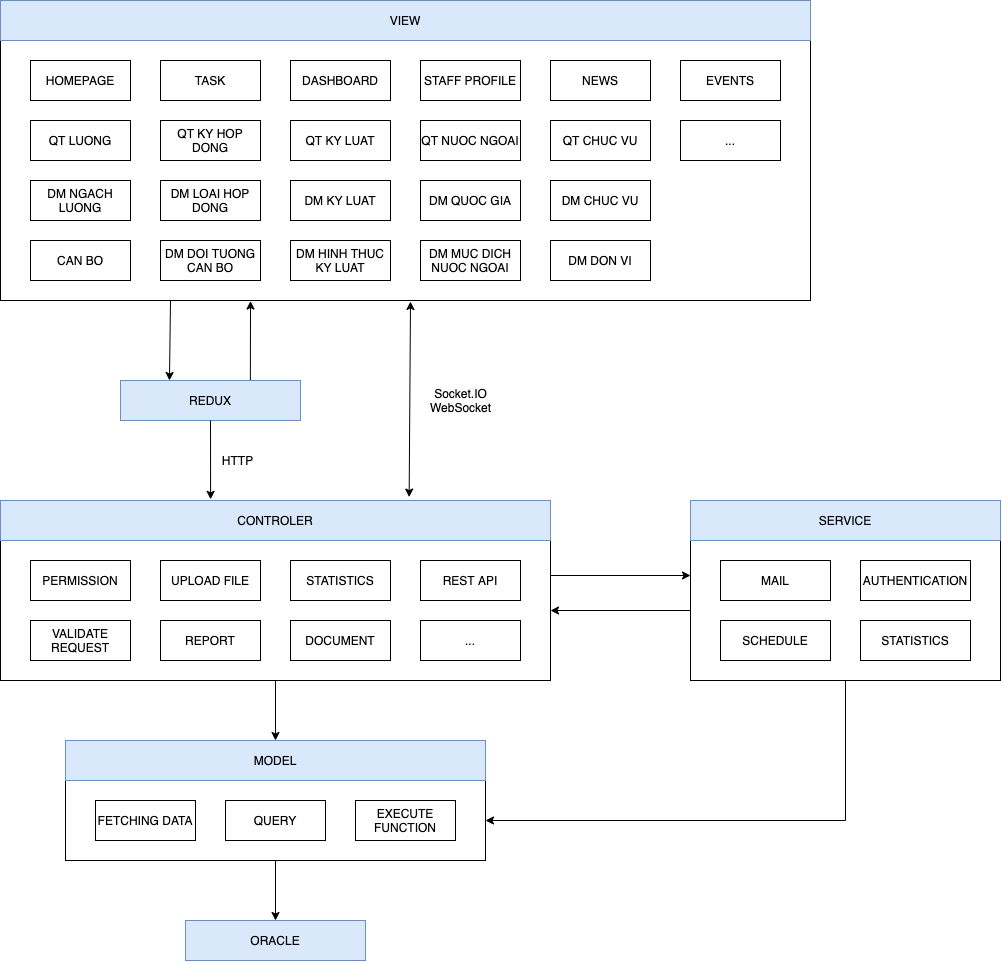
\includegraphics[width=15cm]{img/MVCInTchc.png}
  \captionof{figure}{Kiến trúc tổng thể của hệ thống}
\end{center}
\section{Thiết kế đối tượng người dùng}
\subsection{Danh sách đối tượng người dùng}
Dựa vào những yêu cầu thực tế của hệ thống và những khảo sát thực tế đối với các cá nhân có nhu cầu sử dụng, xây dựng hệ thống Tổ chức - Hành chính. Nhóm đưa ra các vai trò, người dùng chính trong hệ thống như sau:
\begin{table}[H]
    \centering
	\begin{tabular}{|p{1cm}|p{4cm}|p{10cm}|}
    \hline
    \textbf{STT}&\textbf{Người dùng}&\textbf{Đặc tả}\\
    \hline
    1&Khách&Là những người dùng chưa đăng nhập, bao gồm tất cả các đối tượng như cán bộ công nhân viên nhà trường, sinh viên, cựu sinh viên, phụ huynh, đơn vị, doanh nghiệp là đối tác của nhà trường,...
    
    Khách có chức năng xem thông tin, tin tức, sự kiện của nhà trường, gửi email liên hệ, và đăng nhập.\\
    \hline
	2&Cán bộ công nhân viên nhà trường&Người dùng với mục đích quản lý được thông tin, hồ sơ, các quá trình nghiệp vụ của bản thân.\\
	\hline
    3&Cán bộ phòng Tổ chức - Hành chính&Là những cán bộ thuộc phòng Tổ chức - Hành chính. Họ có chức năng quản lý thông tin của các cán bộ, quản lý thông tin các quá trình nghiệp vụ của nhà trường.\\
    \hline
    4&Quản lý phòng Tổ chức - Hành chính (Trưởng phòng, phó phòng) &Chức năng chính là quản lý hệ thống và công việc của các cán bộ thuộc phòng Tổ chức - Hành chính. \\
	\hline
    5&Quản trị hệ thống&Là những người tạo ra hệ thống ban đầu, có các chức năng hỗ trợ tạo ra các cấu hình cho hệ thống, bao gồm các thao tác như: cấu hình các thông tin chung của phòng Tổ chức-Hành chính, cấu hình về giao diện, quản lý tài khoản người dùng\\
	\hline
\end{tabular}
\caption{Danh sách đối tượng người dùng của hệ thống}
\end{table}
\begin{center}
  \captionsetup{type=figure}
  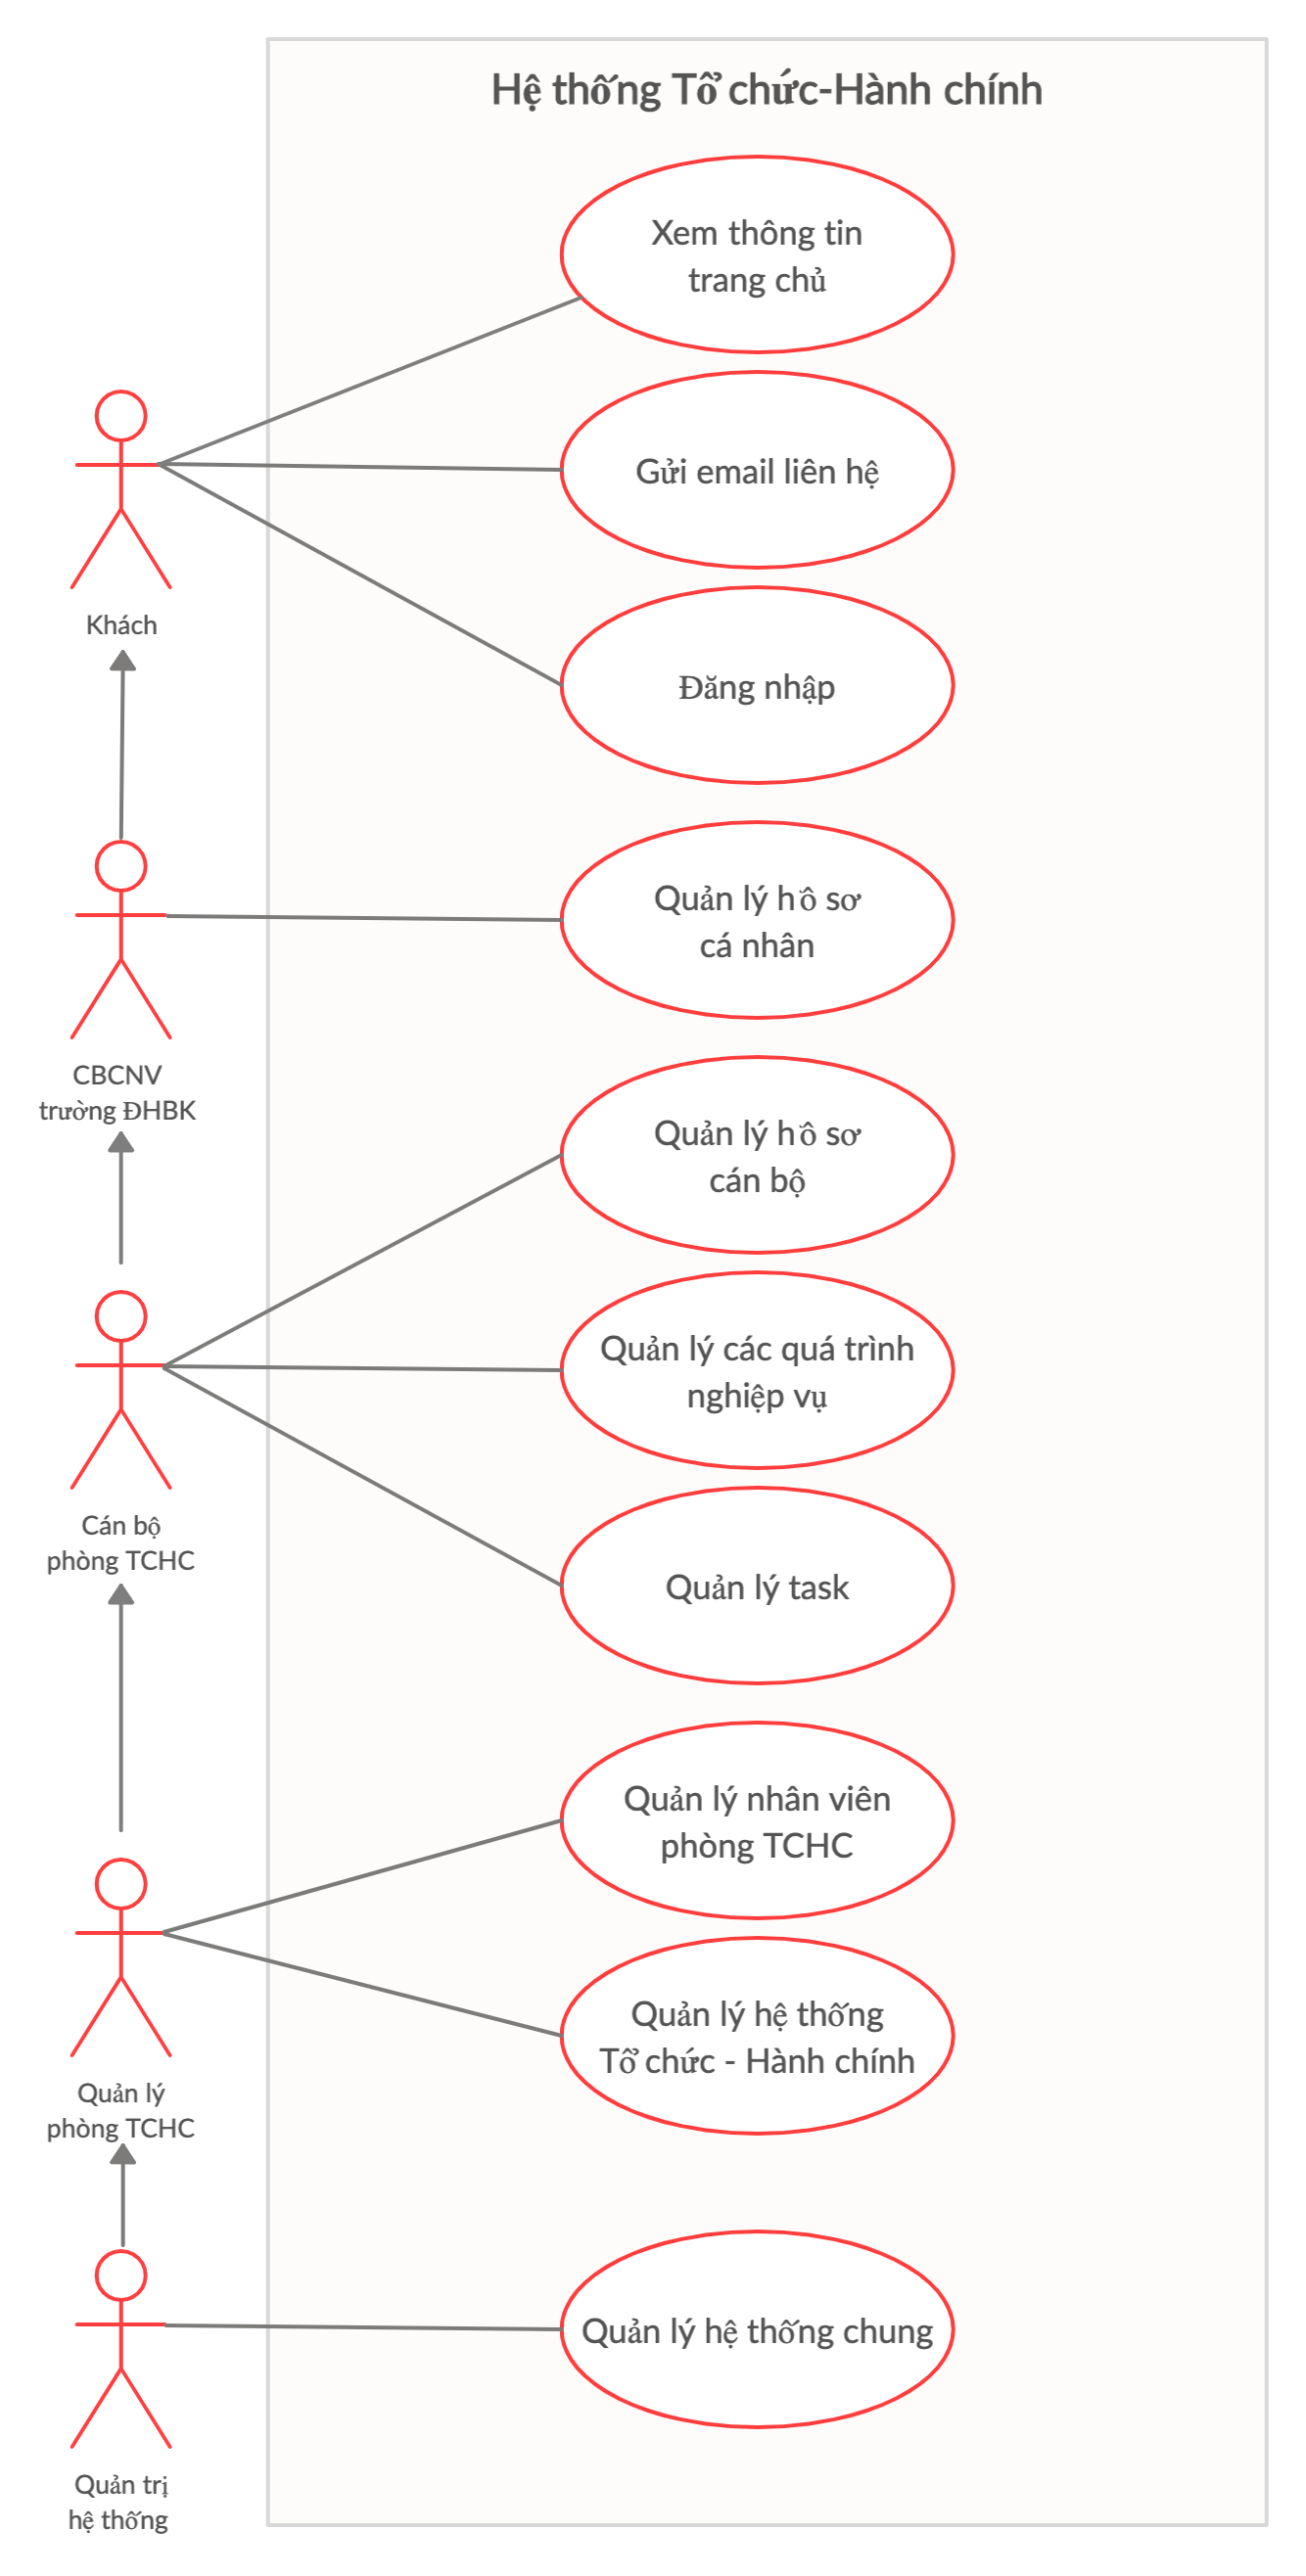
\includegraphics[width=11cm]{img/usecase/rootUsecase.png}
  \captionof{figure}{Lược đồ Usecase các đối tượng của hệ thống }
\end{center}
\subsection{Đối tượng: Khách}
\textbf{Lược đồ Usecase đối tượng khách}
\begin{center}
  \captionsetup{type=figure}
  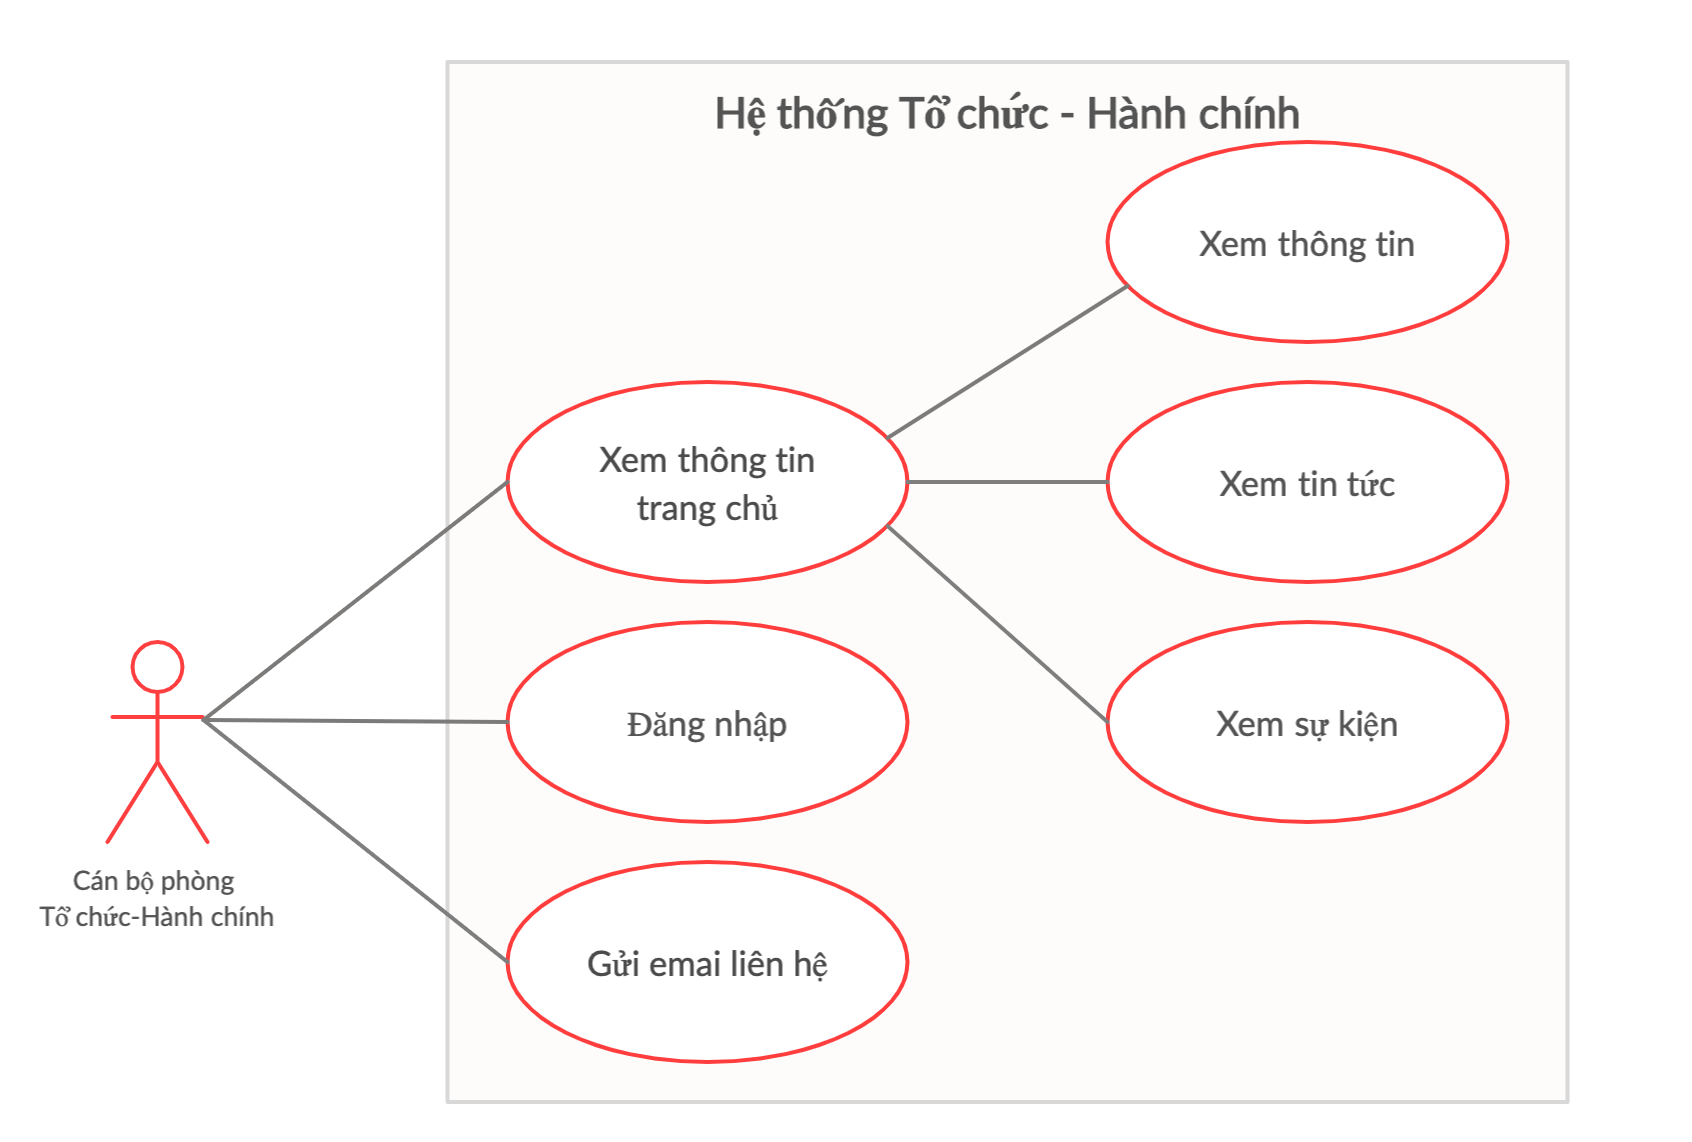
\includegraphics[width=14cm]{img/usecase/guest.png}
  \captionof{figure}{Lược đồ Usecase của đối tượng khách}
\end{center}

Khách là những người dùng chưa đăng nhập, bao gồm tất cả các đối tượng như cán bộ công nhân viên nhà trường, sinh viên, cựu sinh viên, phụ huynh, đơn vị, doanh nghiệp là đối tác của nhà trường,...
 
 Đối tượng khách có thể truy cập trang chủ để xem các thông tin chung, thông tin liên hệ, xem các tin tức và sự kiện. Khi có nhu cầu liên hệ với nhà trường, khách có thể vào mục liên hệ để gửi email đến nhà trường.
 
 Khi khách là cán bộ công nhân viên trường Đại học Bách Khoa Tp.HCM, khách có thể đăng nhập bằng tài khoản email nhà trường cung cấp để sử dụng hệ thống với các vai trò cán bộ nhà trường.

\subsection{Đối tượng: Cán bộ công nhân viên nhà trường}
\textbf{Lược đồ Usecase đối tượng cán bộ của trường}
\begin{center}
  \captionsetup{type=figure}
  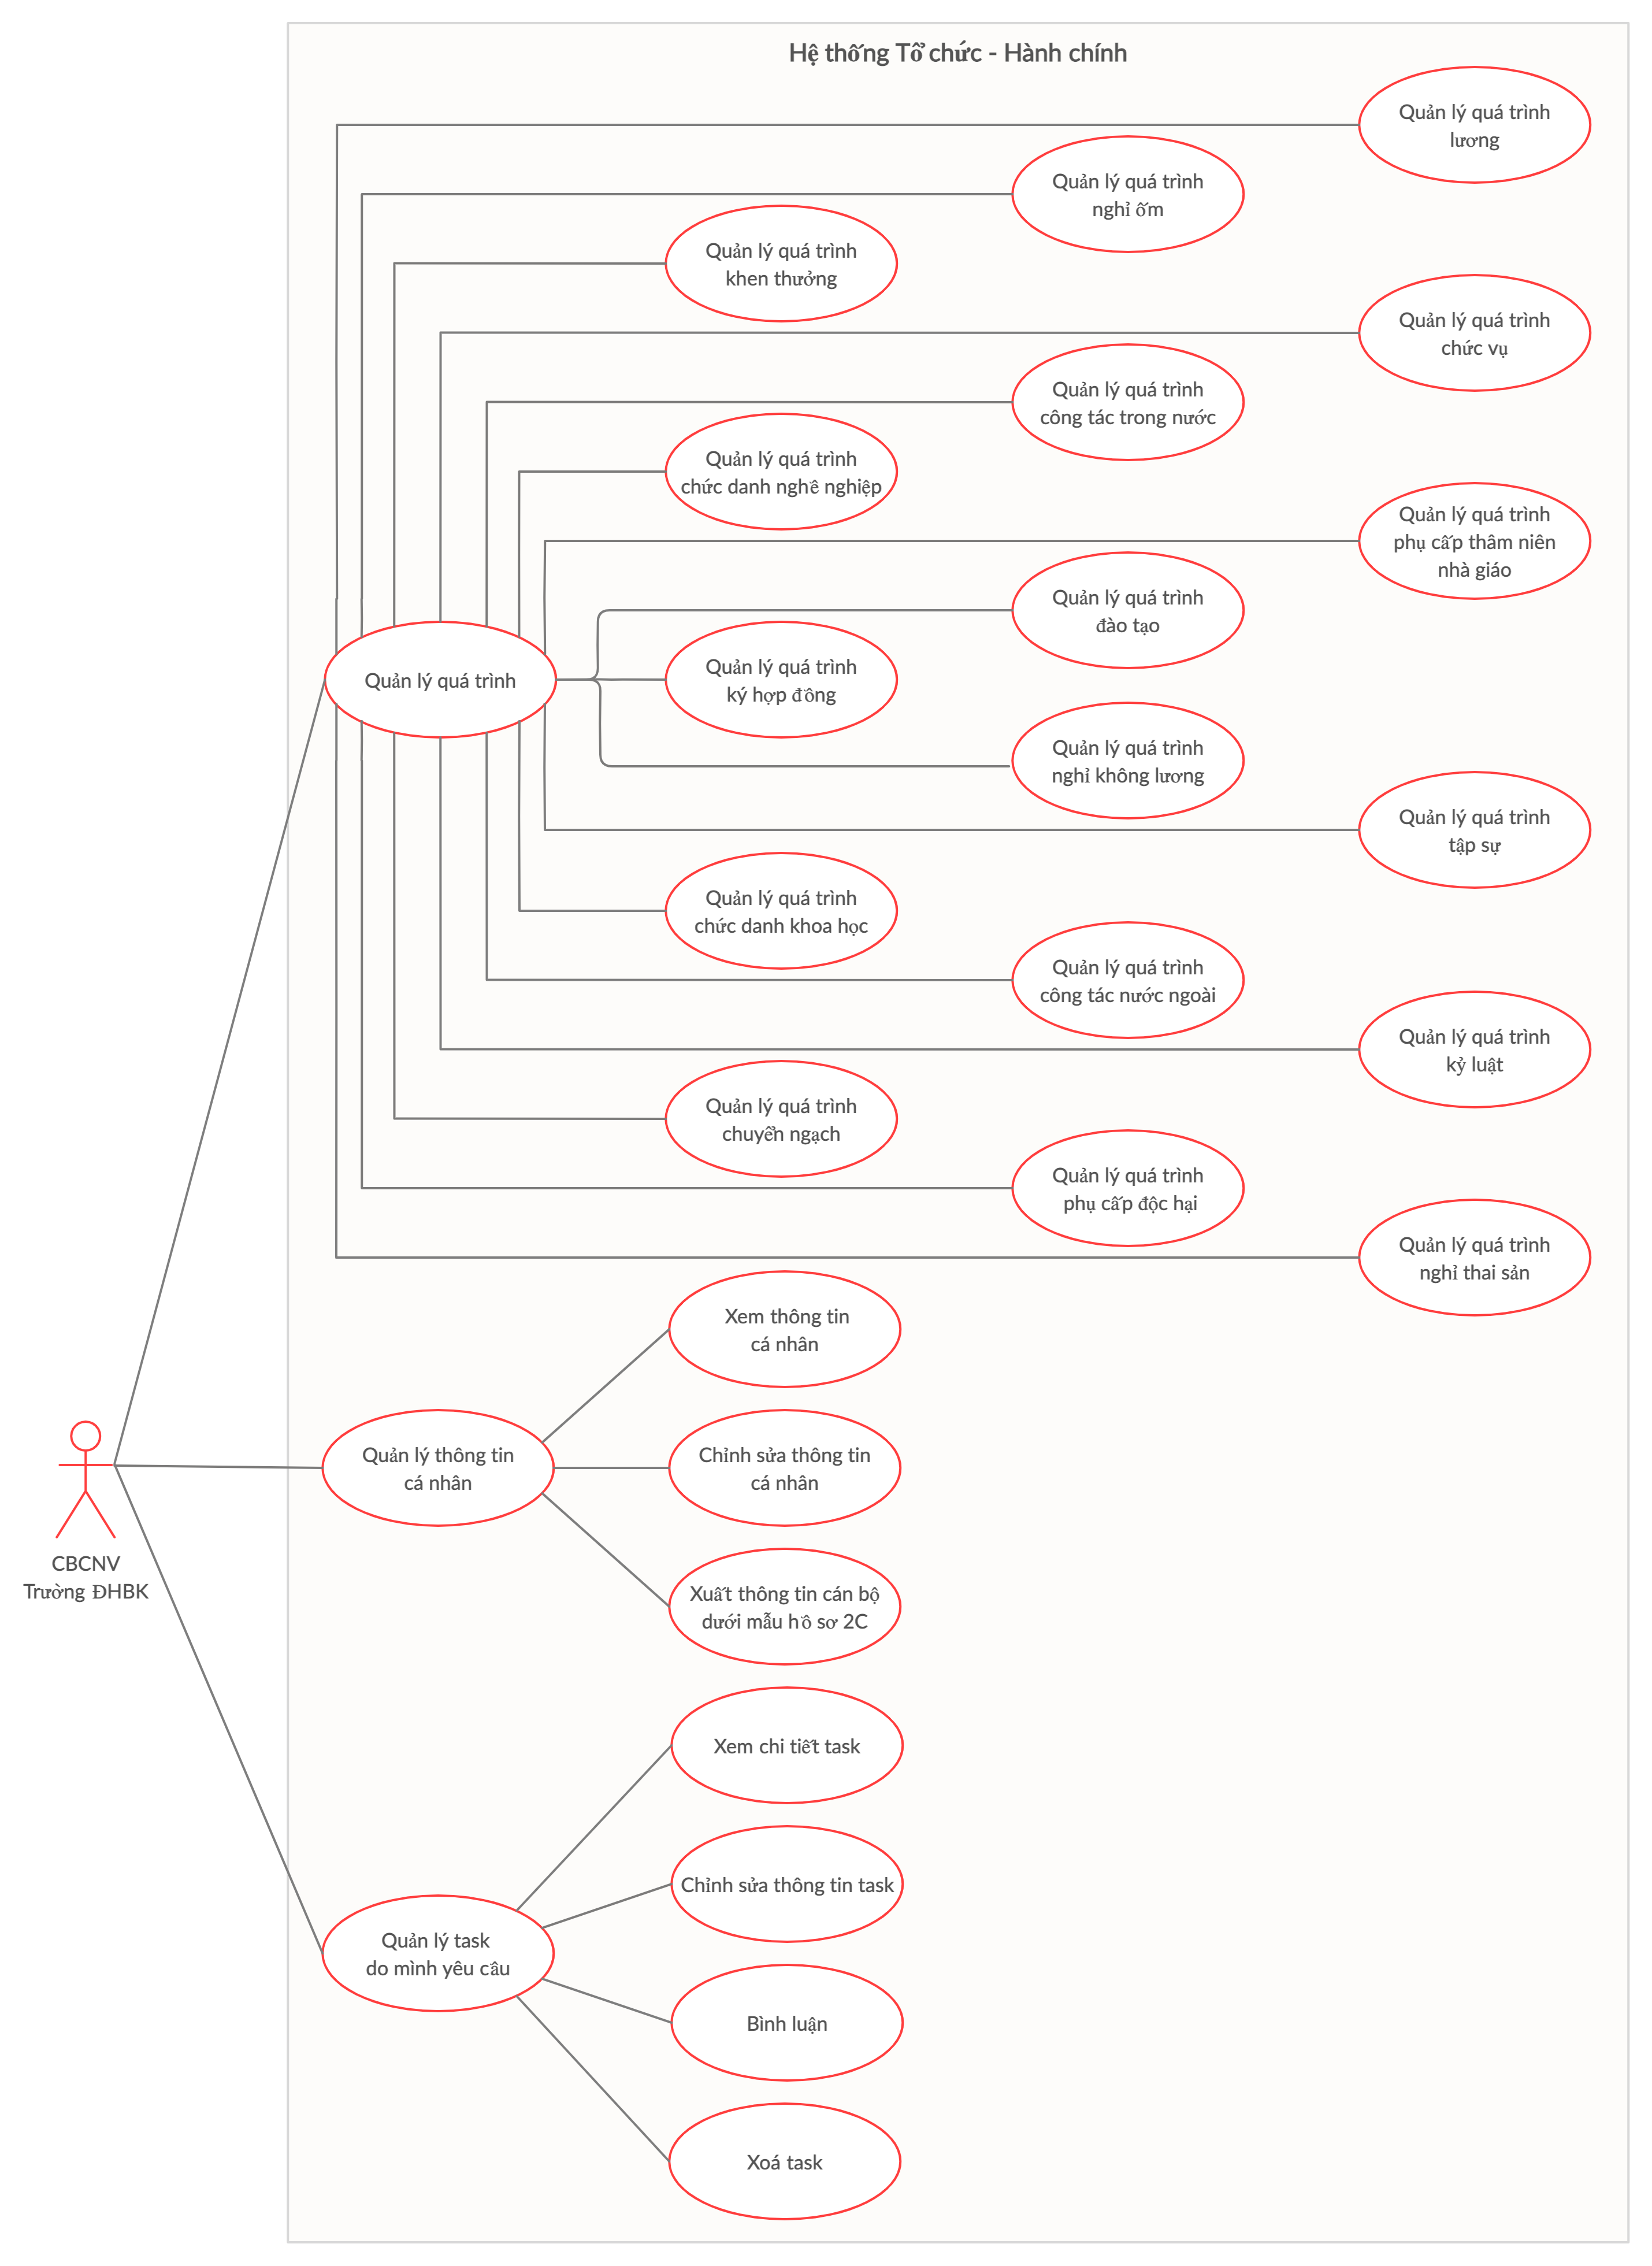
\includegraphics[width=15cm]{img/usecase/userUsecase.png}
  \captionof{figure}{Lược đồ Usecase đối tượng cán bộ công nhân viên nhà trường}
\end{center}

Đối với người dùng là cán bộ của trường, sau khi đăng nhập sẽ có chức năng quản lý thông tin của cá nhân, quản lý các quá trình nghiệp vụ của bản thân.

Quản lý thông tin cá nhân bao gồm xem thông tin, sửa đổi và xuất thông tin theo mẫu sơ yếu lý lịch cán bộ, công chức (Mẫu 2C-BNV/2008).

Cán bộ có thể xem thông tin các quá trình nghiệp vụ của bản thân như quá trình lương, quá trình nghỉ ốm, nghỉ không lương, nghỉ thai sản,... 

Khi muốn tạo mới, sửa đổi hoặc xoá quá trình, cán bộ công nhân viên nhà trường có thể tạo yêu cầu tương ứng để cán bộ phòng Tổ chức - Hành chính xem xét và duyệt yêu cầu.

\subsection{Đối tượng: Cán bộ phòng Tổ chức - Hành chính}
\textbf{Lược đồ Usecase đối tượng cán bộ phòng Tổ chức - Hành chính}
\begin{center}
  \captionsetup{type=figure}
  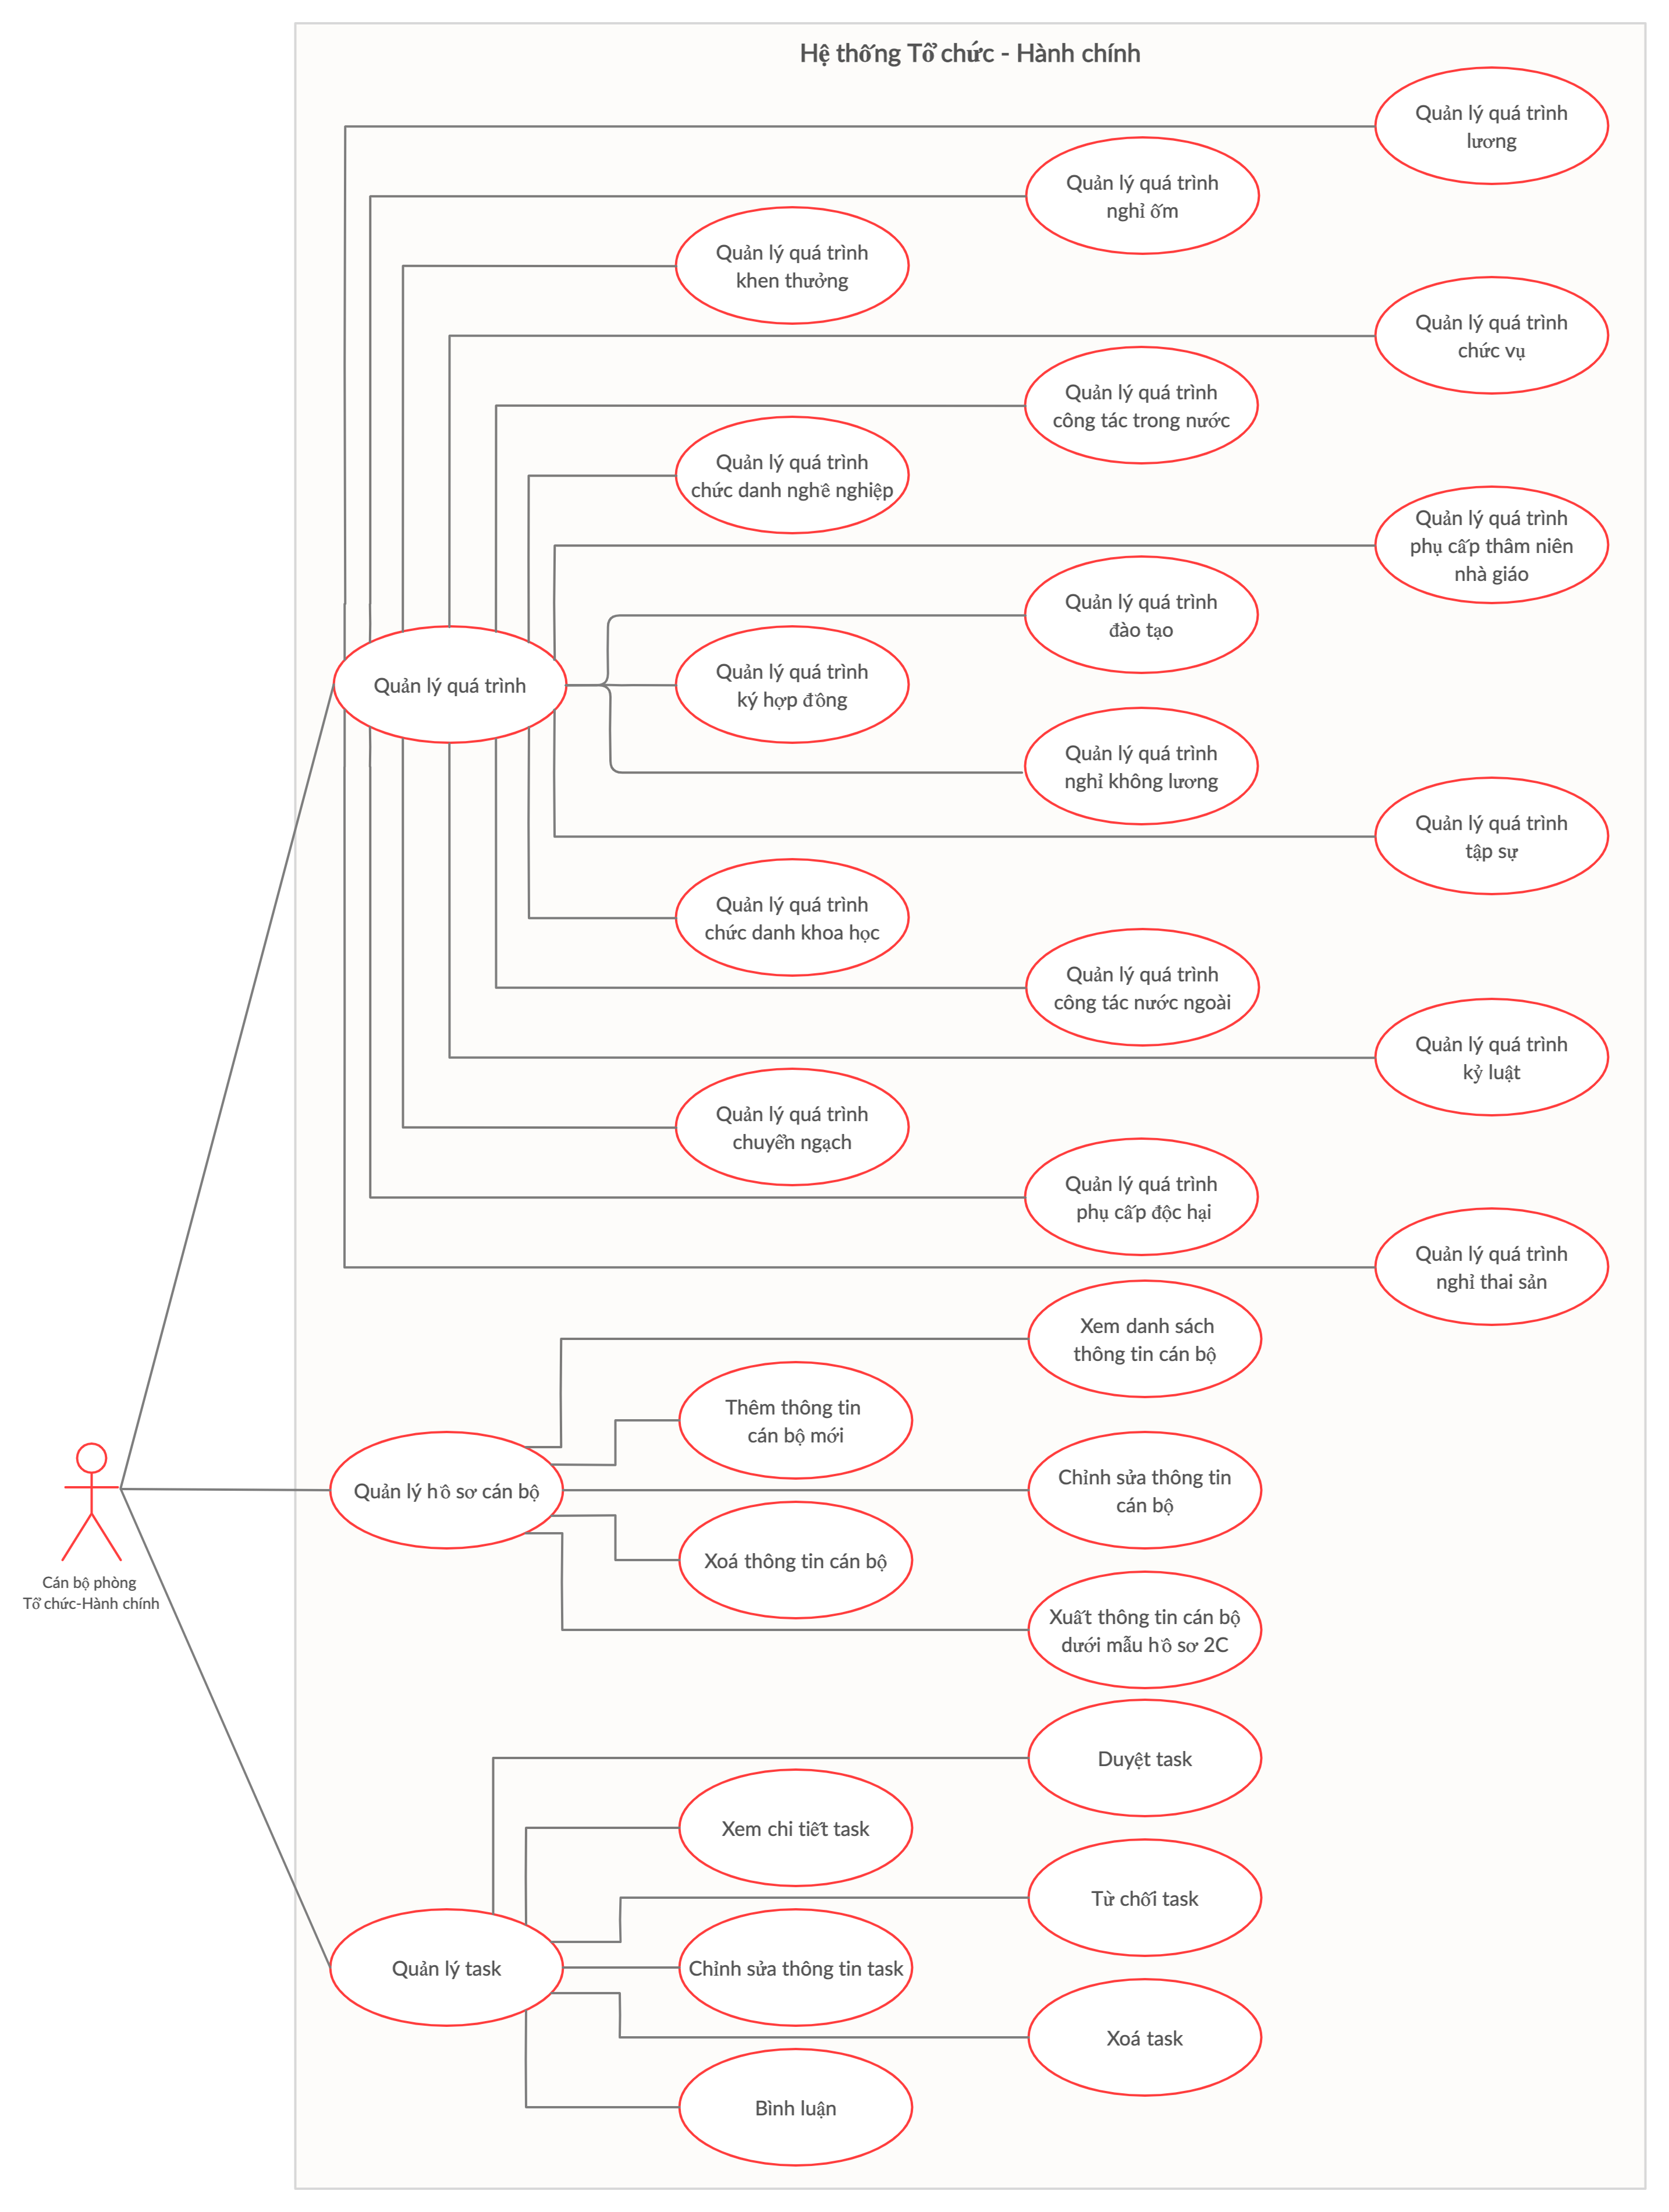
\includegraphics[width=15cm]{img/usecase/nhanVienTCHC.png}
  \captionof{figure}{Lược đồ Usecase đối tượng cán bộ phòng Tổ chức - Hành chính}
\end{center}

Sau khi đăng nhập vào hệ thống, người dùng là cán bộ phòng Tổ chức - Hành chính sẽ có các nhóm chức năng sau: quản lý cán bộ, quản lý các quá trình nghiệp vụ và các yêu cầu của của người dùng.

Chức năng quản lý cán bộ bao gồm xem danh sách toàn bộ cán bộ nhà trường, tạo mới, sửa đổi và xoá cán bộ. Ngoài ra còn có chức năng xuất danh sách cán bộ dưới dạng excel, xuất hồ sơ lý lịch theo mẫu 2C.

Chức năng quản lý các quá trình nghiệp vụ bao gồm xem danh sách các quá trình như quá trình công tác trong nước, quá trình công tác nước ngoài, quá trình lương,... Tạo mới quá trình, chỉnh sửa thông tin quá trình và xoá quá trình.

Cán bộ phòng Tổ chức - Hành chính còn có nhiệm vụ quản lý các yêu cầu của các cán bộ công nhân viên nhà trường, xem xét, chỉnh sửa, bình luận, từ chối và duyệt yêu cầu.

\subsection{Đối tượng: Quản lý phòng Tổ chức - Hành chính}
\textbf{Lược đồ Usecase đối tượng quản lý phòng Tổ chức - Hành chính}
\begin{center}
  \captionsetup{type=figure}
  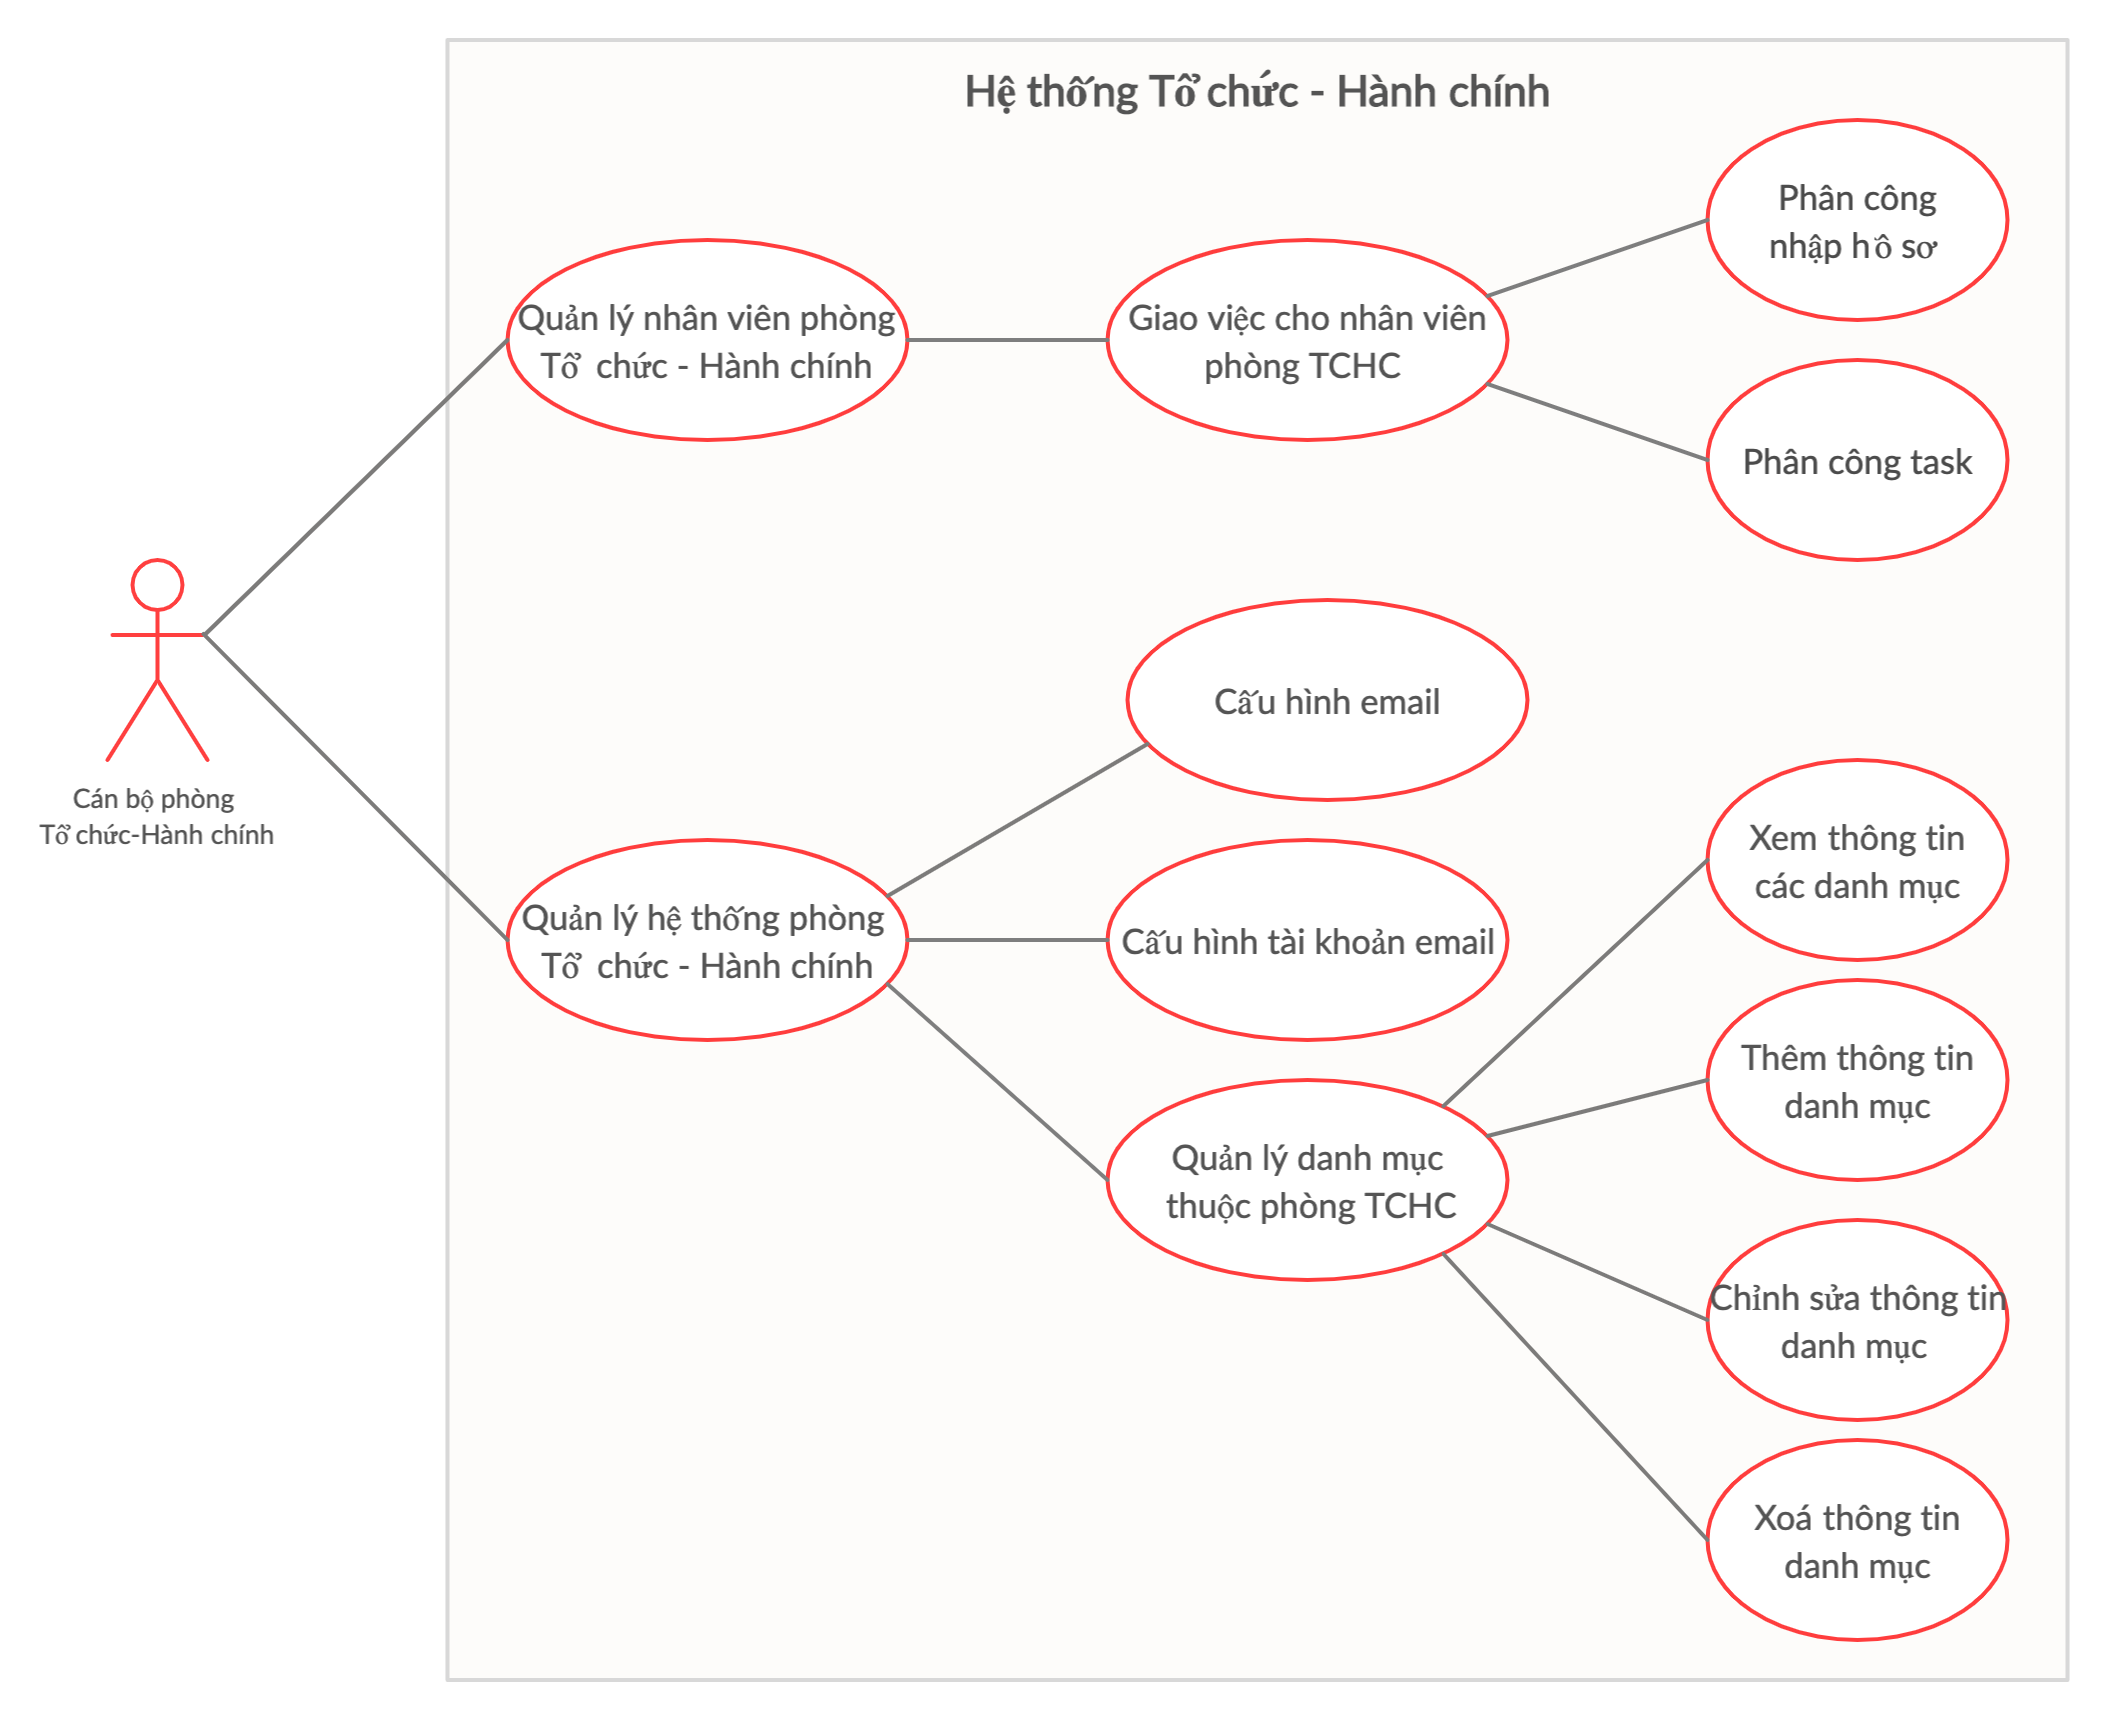
\includegraphics[width=15cm]{img/usecase/quanLyPhong.png}
  \captionof{figure}{Lược đồ Usecase cho đối tượng quản lý phòng Tổ chức - Hành chính}
\end{center}
Quản lý phòng Tổ chức - Hành chính sau khi đăng nhập sẽ có tất cả các nhóm chức năng như trên của cán bộ của phòng Tổ chức - Hành chính và có thêm chức năng quản trị các danh mục, thông tin thuộc phòng Tổ chức - Hành chính.

Bên cạnh đó, quản lý phòng còn có nhiệm vụ phân công công việc cho nhân viên như phân công nhập hồ sơ, phân công duyệt yêu cầu.

\subsection{Đối tượng: Quản trị hệ thống}
\textbf{Lược đồ Usecase đối tượng quản trị hệ thống}
\begin{center}
  \captionsetup{type=figure}
  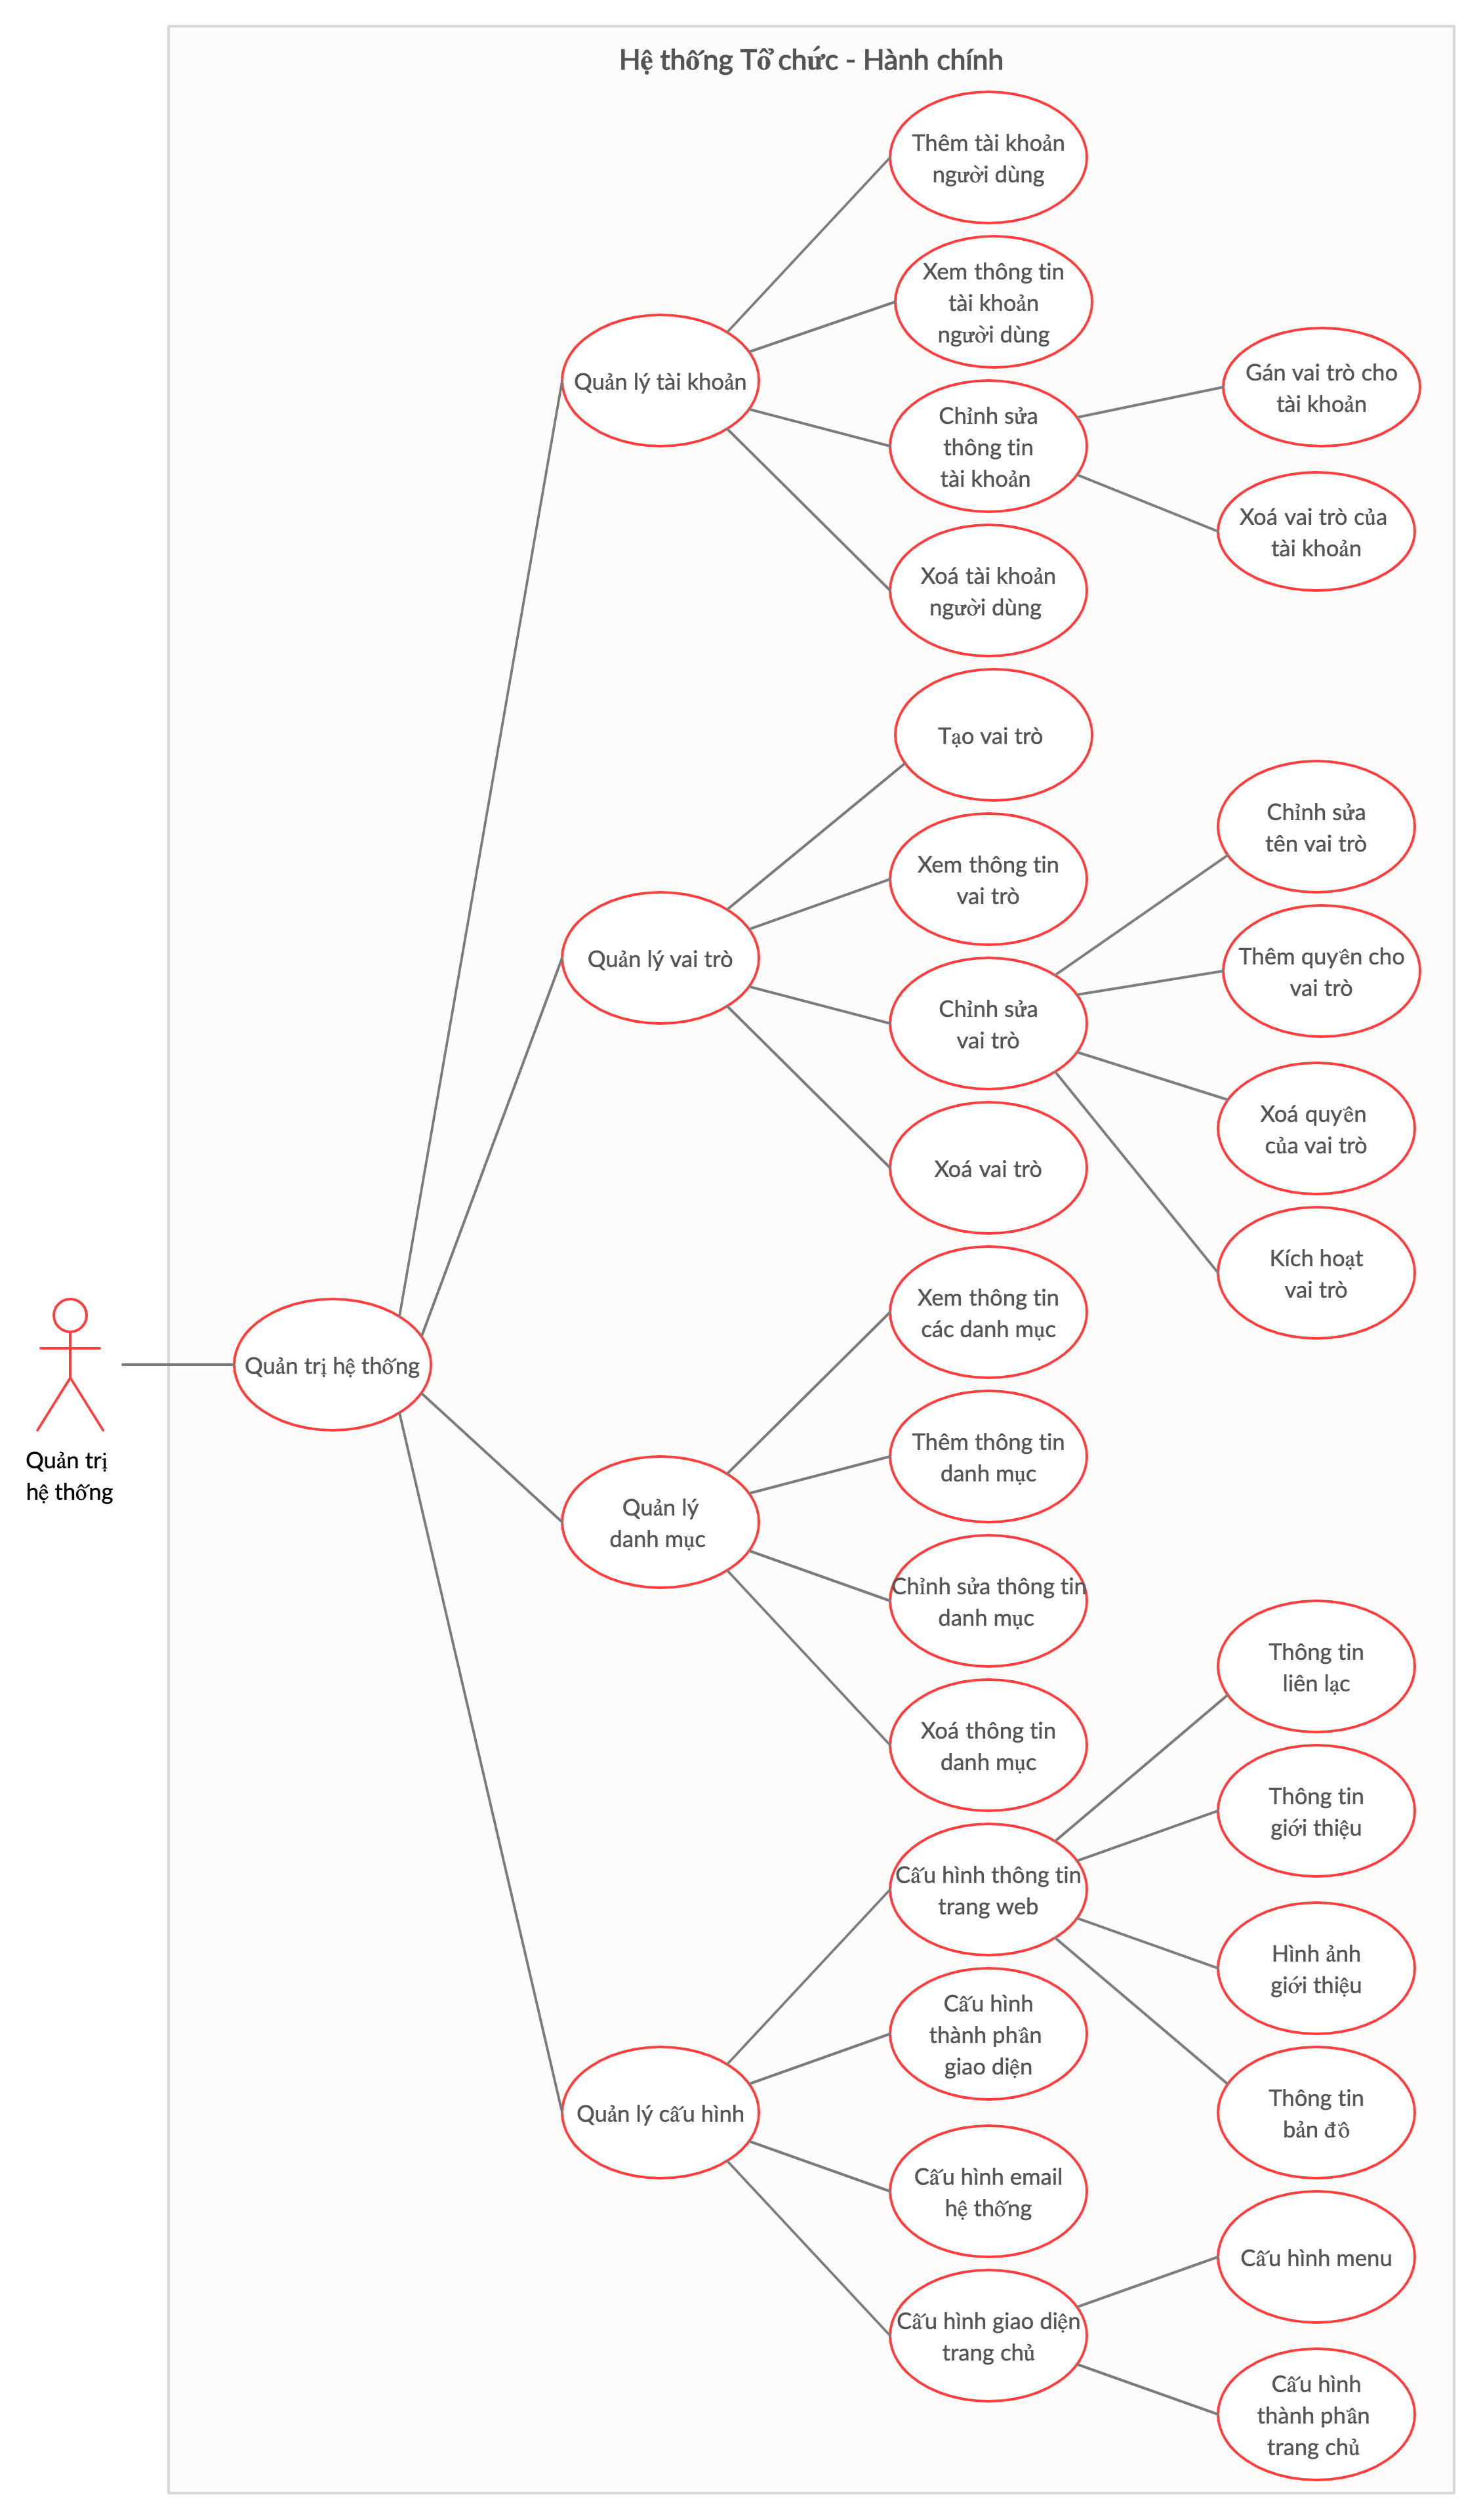
\includegraphics[width=13cm]{img/usecase/admin.png}
  \captionof{figure}{Lược đồ usecase của đối tượng quản trị hệ thống}
\end{center}

\indent Đối với đối tượng là quản trị hệ thống, sau khi xác thực thành công sẽ có những nhóm chức năng: quản lý tài khoản, quản lý vai trò, quản lý danh mục và quản lý cấu hình. Với mỗi nhóm chức năng sẽ có những chức năng tương ứng sau:

\begin{itemize}
    \item Nhóm quản lý tài khoản bao gồm các chức năng:
        \subitem - Xem thông tin các tài khoản.
        \subitem - Tạo mới tài khoản.
        \subitem - Xoá tài khoản người dùng.
        \subitem - Chỉnh sửa thông tin tài khoản.
        \subitem - Thêm và xoá vai trò cho tài khoản.
    \item Nhóm quản lý vai trò bao gồm các chức năng:
        \subitem - Xem danh sách các vai trò.
        \subitem - Tạo mới và xoá vai trò.
        \subitem - Kích hoạt vai trò.
        \subitem - Thêm và xoá quyền cho vai trò.
    \item Chức năng quản lý danh mục là chức năng xây dựng và sửa đổi thông tin những danh mục mặc định phục vụ cho việc nhập và lữu trữ dữ liệu trong hệ thống.
    \item Nhóm quản lý cấu hình gồm các chức năng: cấu hình giao diện trang chủ, cấu hình thông tin trang web, cấu hình email cho hệ thống.
        \subitem - Cấu hình giao diện trang chủ: Tùy chỉnh các thành phần giao diện, lựa chọn các thành phần giao diện sẽ xuất hiện ở trang chủ.
        \subitem - Cấu hình thông tin trang web: Cấu hình các thông tin chung cho hệ thống, thông tin liên lạc của phòng Tổ chức - Hành chính.
        \subitem - Cấu hình email hệ thống: Tủy chỉnh các mẫu email tự động của hệ thống.
\end{itemize}
\section{Thiết kế cơ sở dữ liệu cho hệ thống}
\subsection{Lược đồ ERD}
\subsection{Lược đồ cơ sở dữ liệu}
\begin{center}
  \captionsetup{type=figure}
  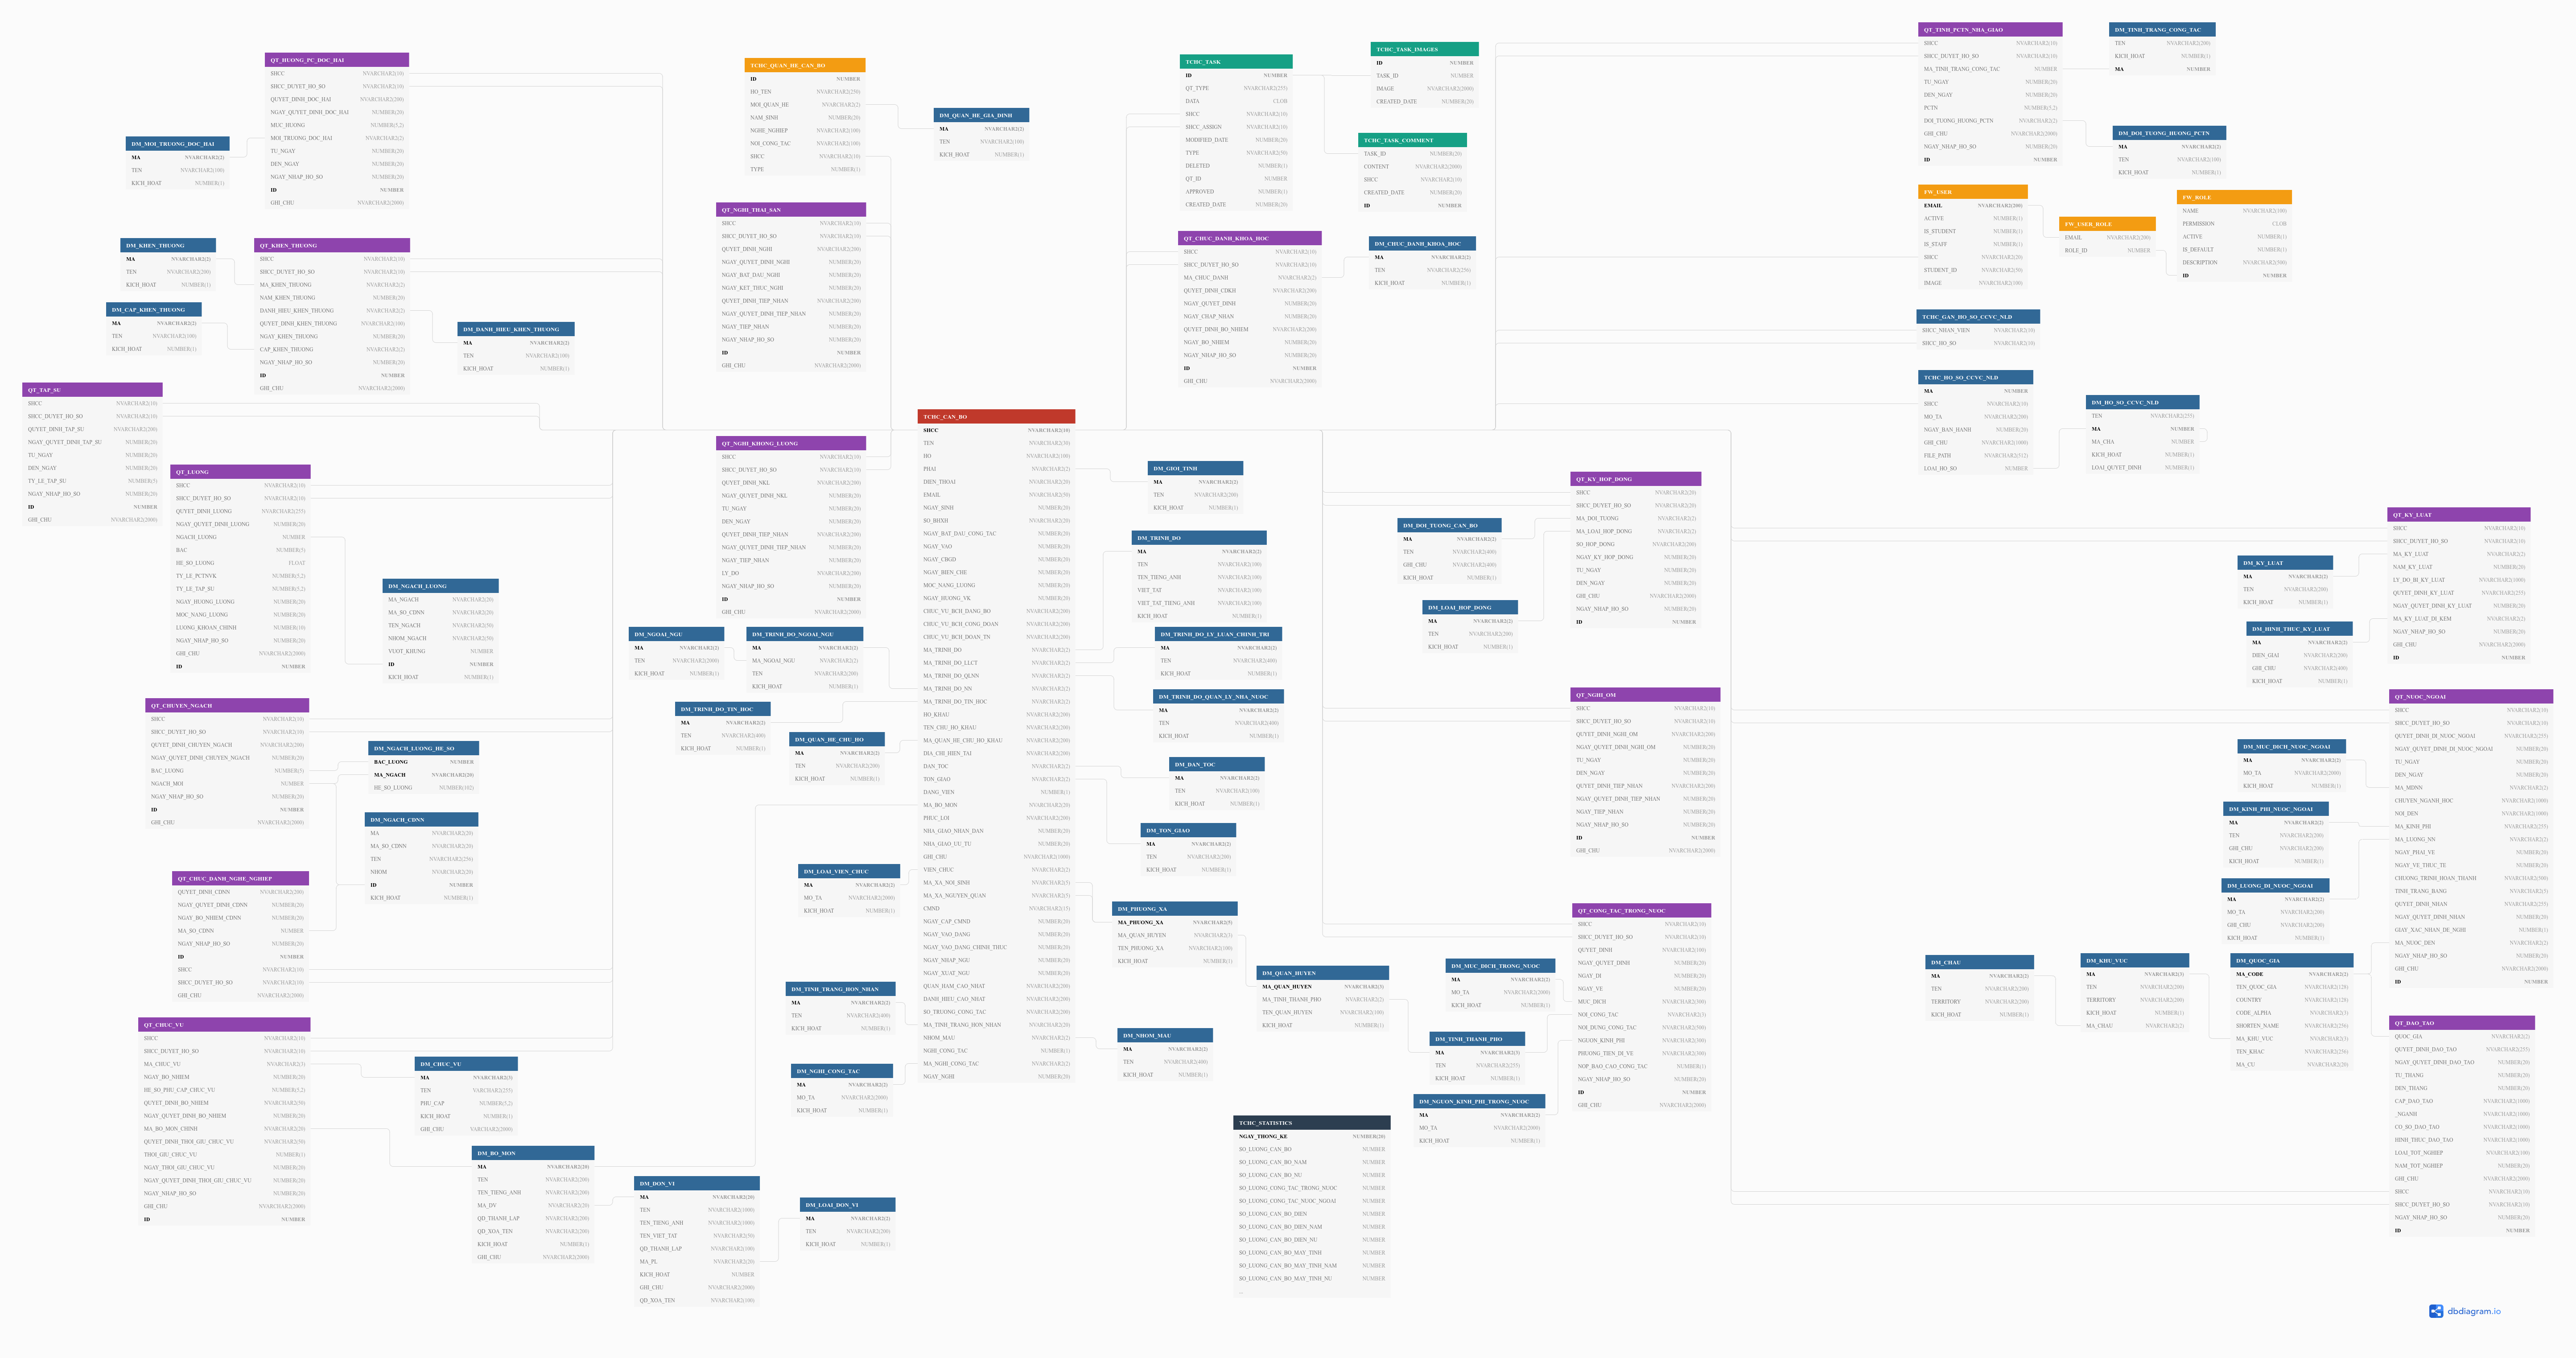
\includegraphics[width=15cm]{img/Screen/dbdiagram.png}
  \captionof{figure}{Thiết kế cơ sở dữ liệu của hệ thống}
\end{center}
Chi tiết xem ở tài liệu đính kèm.